\documentclass[main.tex]{subfiles}
\begin{document}
    \section{Propulsion}
    Propulsion, the new challenge for Competition III, is the most challenging subsystem to design, and its design additionally dictates the design of every other component on the pod. To select the best possible method of propulsion given competition constraints, we conducted a series of preliminary analyses on possible propulsion designs, the most promising of which were the Friction Drive and Linear Induction Motor (LIM). We eventually chose to invest fully into the Friction Drive design, due to the complexity, mass, and cost of a LIM suited for competition accelerations. [2-3 SUMMARY SENTENCES ABOUT FRICTION]. Friction drive serves as a safe and reliable form of propulsion as it is well researched and tested in many different fields.

    \subsection{Propulsion Feasibility \& Design Candidates}
    We investigated several different methods of propulsion, including chemical propulsion, railgun propulsion, air pressure propulsion, and others. For safety, mass, and cost reasons, our most promising designs were friction drive and linear induction motor. Our initial design, submitted for the Preliminary Design Package, included a LIM.\\

    However, later calculations based on commercially available LIMs showed that off-the-shelf products would be abysmally unsuited for the Hyperloop competition; most such LIMs have a very narrow operating range of velocity, outside of which the motor becomes extremely inefficient. First-principles analysis based on [PAPERS?] showed some promise, but this would require a ground-up design of a variable-pitch linear induction motor, which seems to be on the current cutting edge of linear motor research.\\

    [some kind of diagram or numbers about this @Ben]\\

    We decided to table the LIM design, due to the relative inexperience of our team with electromagnetic propulsion, as well as the very high mass and cost. We do, however, plan to continue researching this to be ready for next year’s competition. Friction drive, though it does not scale well to Hyperloop speeds, will still allow us to gain experience with high power systems and high speed stability and braking systems.\\

    \subsection{Overall Design}
    Full labeled detailed CAD\\
    Mass, power, etc.\\
    Full cost breakdown, comments on manufacturability and production costs\\
    “A full Bill of Materials can be found in Appendix C.”

    \subsection{Structural}
    What are several reasonable and edge-case loading scenarios, and how does the FEA look for all of those? Justify your “reasonable” scenarios. If possible to simulate, how many cycles might it withstand?\\

    How will we deal with stability despite imperfections and irregularities in the track, and resulting modes of vibration? (Simulation would be good)

    \begin{figure}[H]
        \centering
        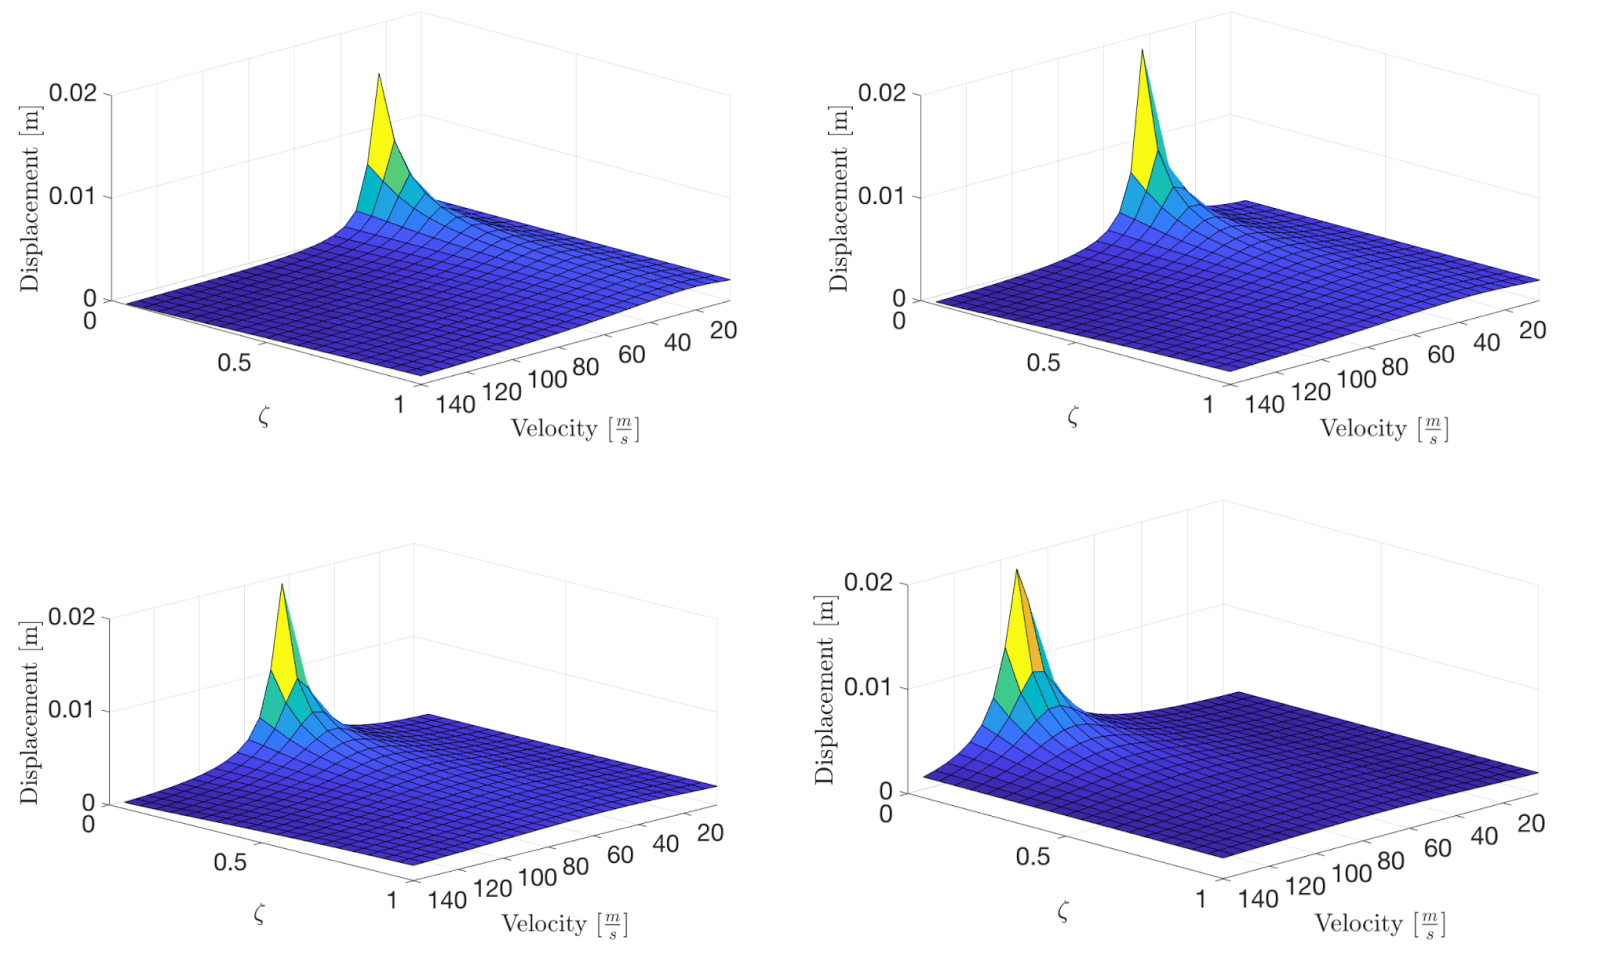
\includegraphics[width=\textwidth]{images/fig1}
        \caption{Spring constant of a. 100,000, b. 250,000, c. 500,000, and d. 1,000,000}
    \end{figure}

    \begin{figure}[H]
        \centering
        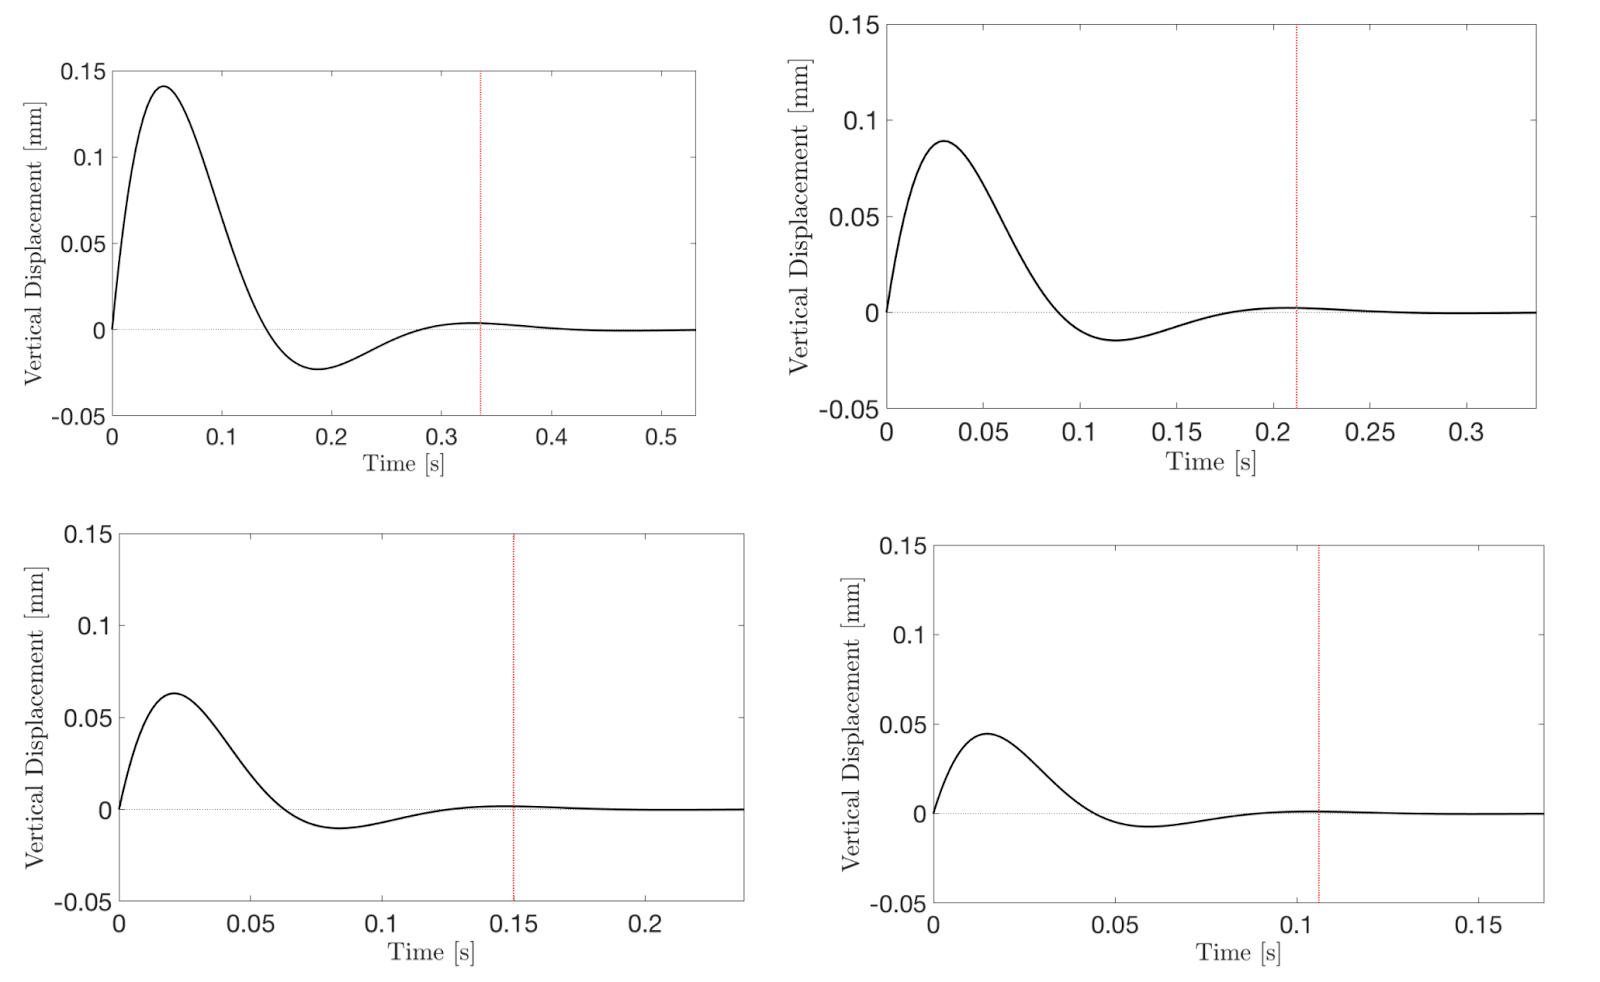
\includegraphics[width=\textwidth]{images/fig2}
        \caption{Spring constant of a. 100,000, b. 250,000, c. 500,000, and d. 1,000,000}
    \end{figure}
    We performed two separate vibrational analyses, in the vertical and horizontal directions, with two separate vibrational damping systems. Based on the construction of the track, the horizontal direction will likely be by far the most problematic; this analysis is detailed in the Lateral subsystem. The vertical damping system is closely integrated into the friction drive system, and so is described here.\\

    First, to determine design parameters of the springs and dampers, several simulations were performed. Different spring constants were chosen, and simulations for each were created using MatLab. The simulated pod was excited with a sinusoidal displacement, with amplitude as the maximum I-beam height tolerance and frequency matching the rate of I-beams passing by the pod. The magnitude of the maximum resulting pod displacement from the beam was plotted for each value of damping coefficient and speed (Figure 1). This series of plots shows the most dangerous combinations of damping coefficient and velocity. For each value of the spring coefficient, as the damping is increased, the vibrations become less intense. It was decided that a value of damping coefficient between [0.5 - 1.0] would be optimal in order to reduce pod vibrations.  Moving forward with this analysis, the response of the pod to a sudden displacement step was measured for a damping coefficient of 0.5 with varying spring constants. This is shown in figure ii. It can be seen that as the spring coefficient is increased, the pod returns to the initial position much faster, which is shown by the red line. Also, as the spring coefficient is increased, the maximum displacement also decreases. Therefore, it was decided that the spring coefficient and damping coefficient should have values of 500,000? And 0.5? Respectively.
    \begin{figure}[H]
        \centering
        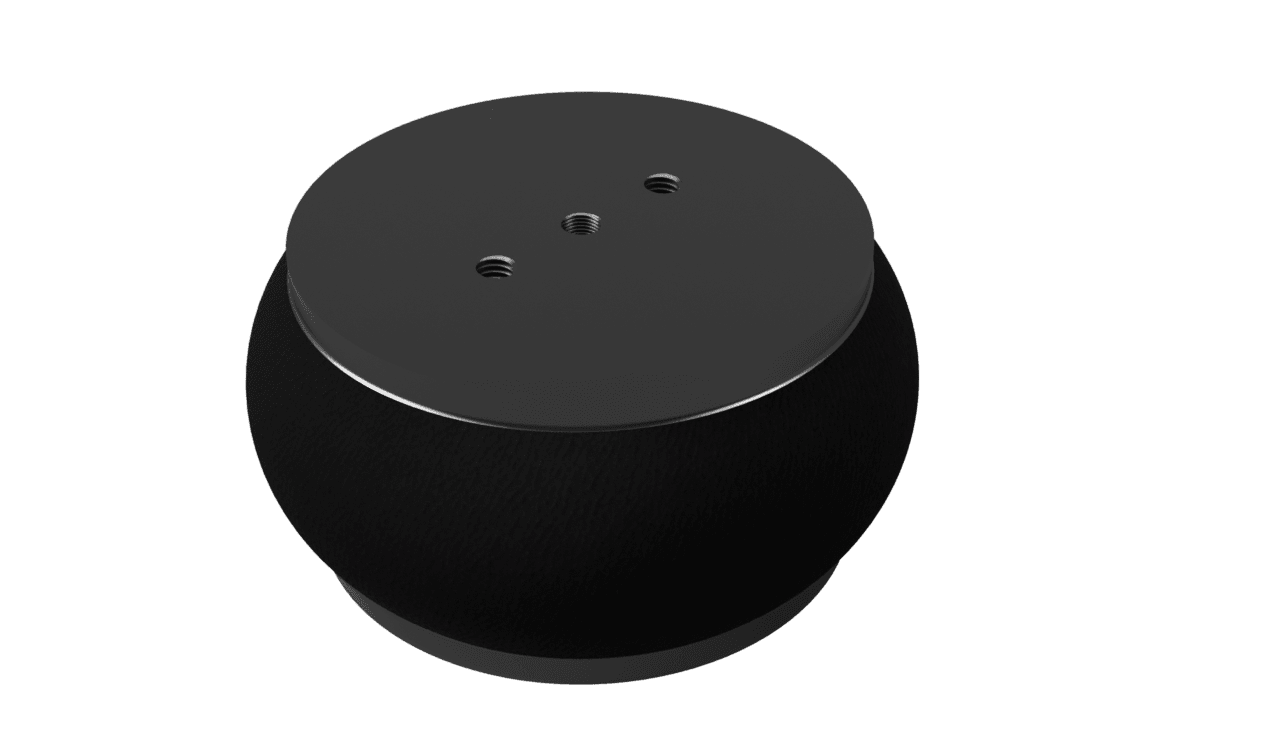
\includegraphics[width=\textwidth]{images/fig3}
        \caption{Caption needed}
    \end{figure}
    The motor-wheel assembly is mounted to the frame using airbag suspension and a Watts linkage. The motor and wheel are isolated from the frame as one unit to avoid the use of a belt tensioner, as the motor and wheel move in unison. Airbags were chosen for their easy adjustability via air pressure and their ability to take high loads.  A Watts linkage allows the unit to move in the normal axis relative to the frame while remaining secured in both the lateral and longitudinal axes.\\

    The material for structural members of the friction drive is Aluminum 6061-T6, chosen for its ease of machinability and high strength to weight ratio. The disadvantages of aluminum in its difficulty of welding was a non-issue, as the structure was not designed to have welded joints.\\

    Add FEA, explain forces and BC\\
    Maybe add properties of 6061? AZ did it\\
    There’s some calcs we can do with max tension / compression of those linkage rods\\

    Mention factors of safety for everything

    \subsection{Motor}
    Comments on why we selected the motor we did\\

    We investigated different types of electric motors to select one that was best suited for our applications, primarily AC induction motors and DC brushless motors. Specifically, axial flux motors were favoured due to their high power density and efficiency. These motors are very light and can provide high torque and power with low heat loss.\\

    It came to several choices of motors from electric motor manufacturers, YASA and EMRAX, that specialize in producing commercial axial flux motors. Several product criteria that affected this choice included:

    \begin{itemize}
        \item Specific power density
        \item RPM range
        \item Torque and power profiles
        \item Efficiency/Thermal Generation
        \item Mass
        \item Power consumption
        \item Cost
    \end{itemize}

    Based on these criteria, the EMRAX 268 was chosen.\\

    EMRAX 268 Specifications
    \begin{figure}[H]
        \centering
        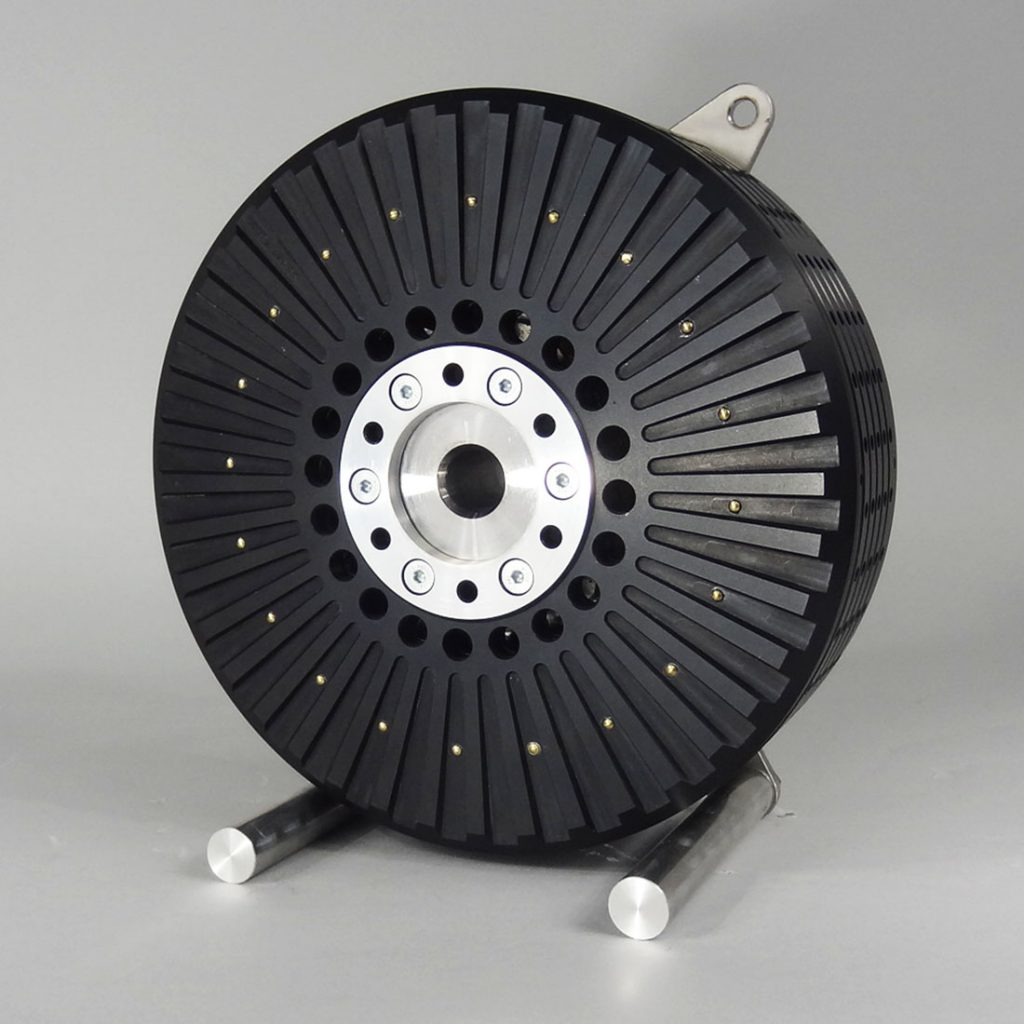
\includegraphics[width=0.5\textwidth]{images/fig4}
        \caption{Side profile of EMRAX 268 Axial Flux Electric Motor}
    \end{figure}
    \begin{figure}[H]
        \centering
        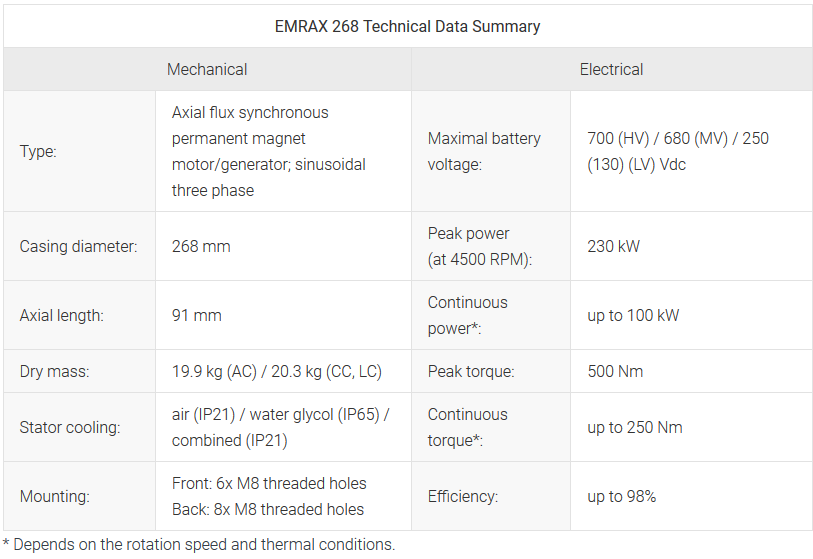
\includegraphics[width=\textwidth]{images/fig5}
        \caption{Summary of EMRAX 268 motor technical data [1]}
    \end{figure}
    \begin{figure}[H]
        \centering
        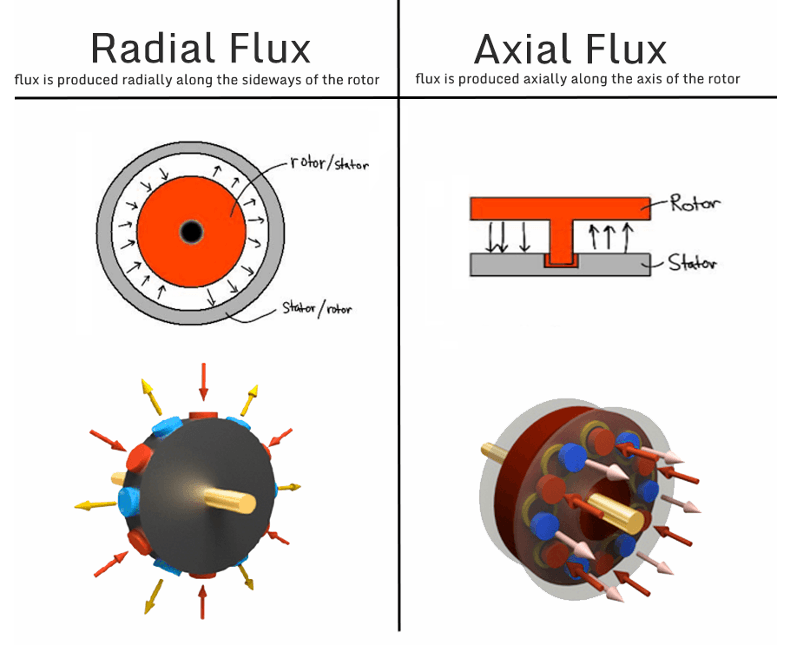
\includegraphics[width=\textwidth]{images/fig6}
        \caption{Axial Flux Motors are built similarly in the same fashion that regular permanent magnet motors are. However, the positions of the stator and rotors are reversed, where the outer casing is the rotor and the inner core is the stator. In addition, most electric motors are radial flux motors where the magnetic flux is oriented along the radial of the stator. Axial flux, as said in the name, orient their magnetic flux axially around the axis of the rotor [2]}
    \end{figure}
    \begin{figure}[H]
        \centering
        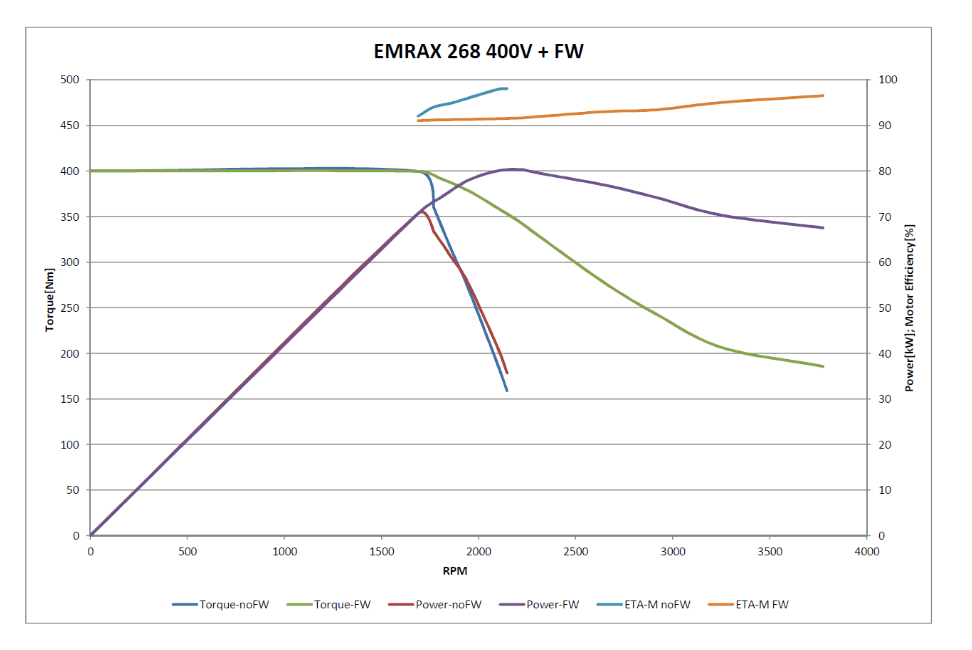
\includegraphics[width=\textwidth]{images/fig7}
        \caption{EMRAX 268 Torque/Mechanical Power/ Efficiency over RPM [3]}
    \end{figure}
    \subsubsection{Motor Performance}
    The graph above shows the torque, power and efficiency of the motor over RPM. As mentioned previously, the motor is capable of producing instantaneous torque, a peak of 400 Nm can be seen in the graph. EMRAX states that the motor is capable of greater RPM ranges by utilizing MFW (magnetic field weakening). The effect of MFW is significant in reducing the decay of torque at higher RPM ranges, and producing higher mechanical power. This is accomplished by reducing the overall efficiency of the motor. However, the reduction is not significant (<8\% greater loss), and the gains in performance outweigh the loss in efficiency.
    \begin{figure}[H]
        \centering
        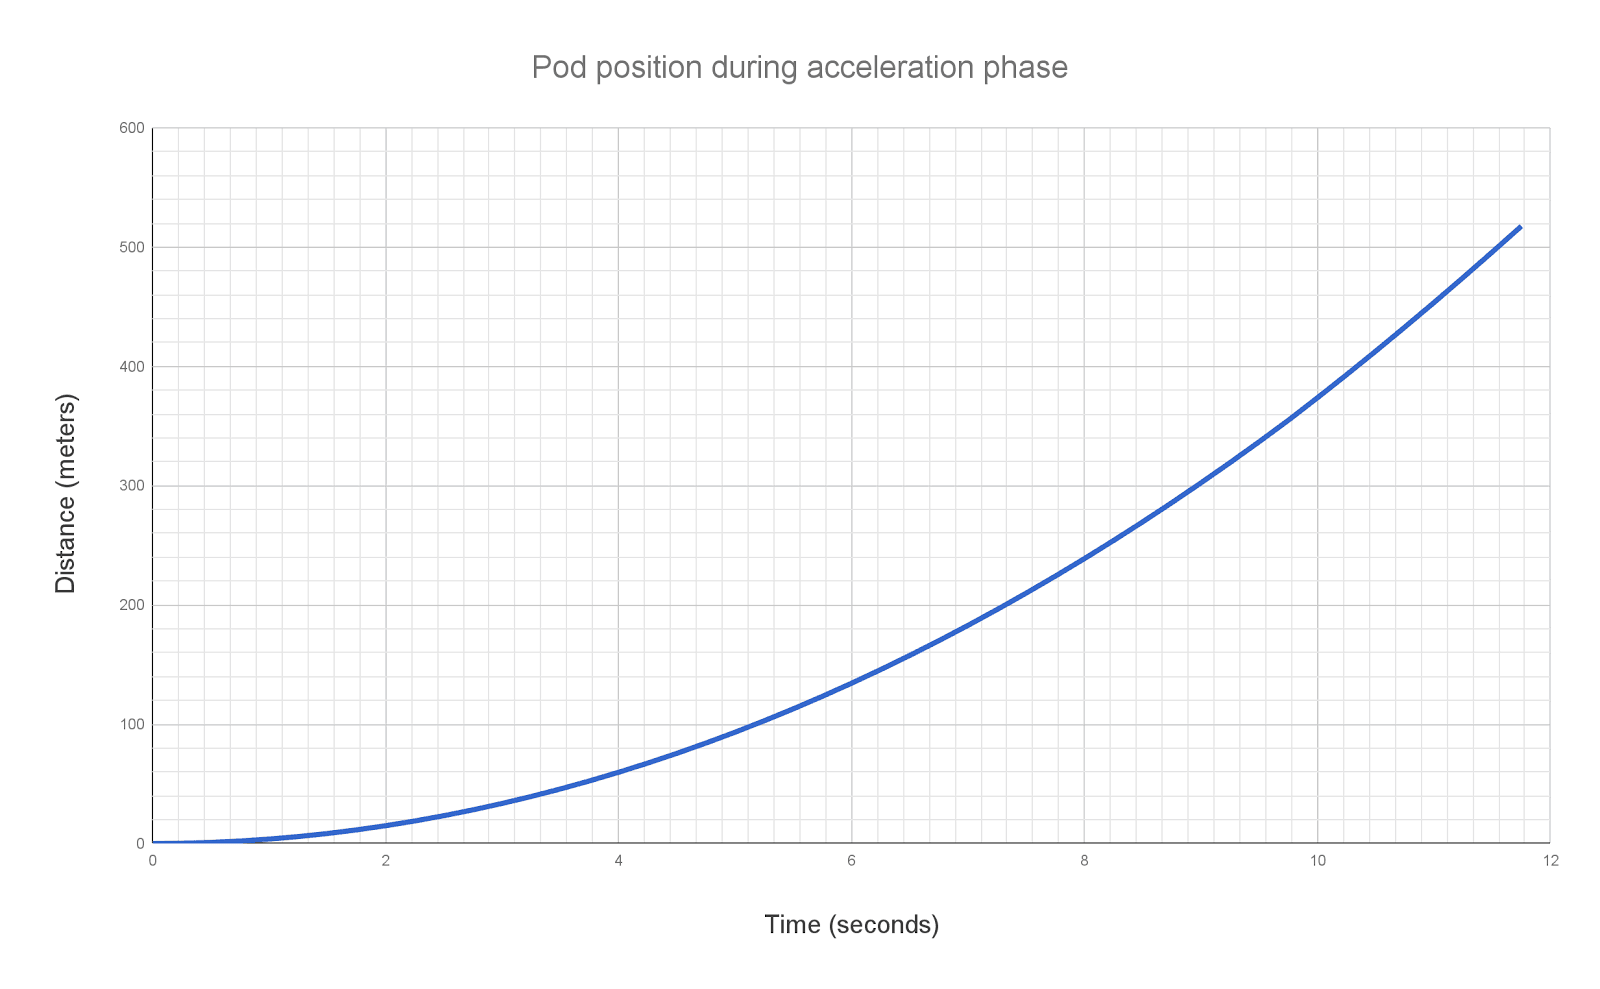
\includegraphics[width=\linewidth]{images/fig8}
        \caption{Pod position during acceleration phase}
    \end{figure}
    \begin{figure}[H]
        \centering
        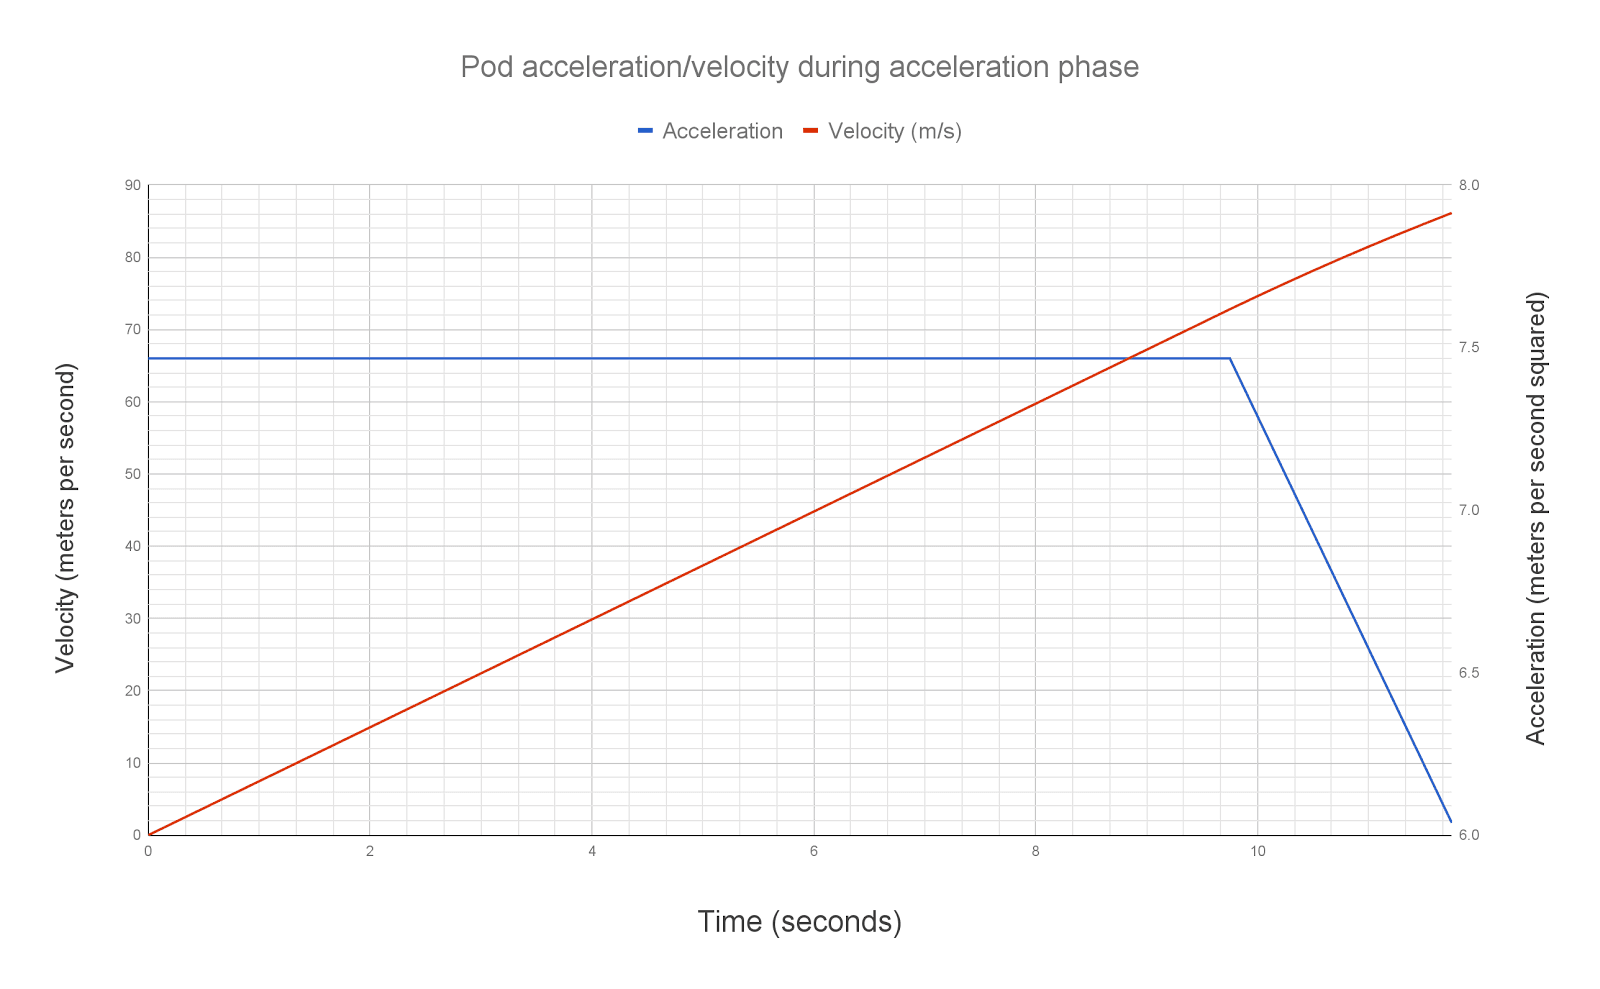
\includegraphics[width=\linewidth]{images/fig9}
        \caption{Pod acceleration/velocity during acceleration phase}
    \end{figure}
    \begin{figure}[H]
        \centering
        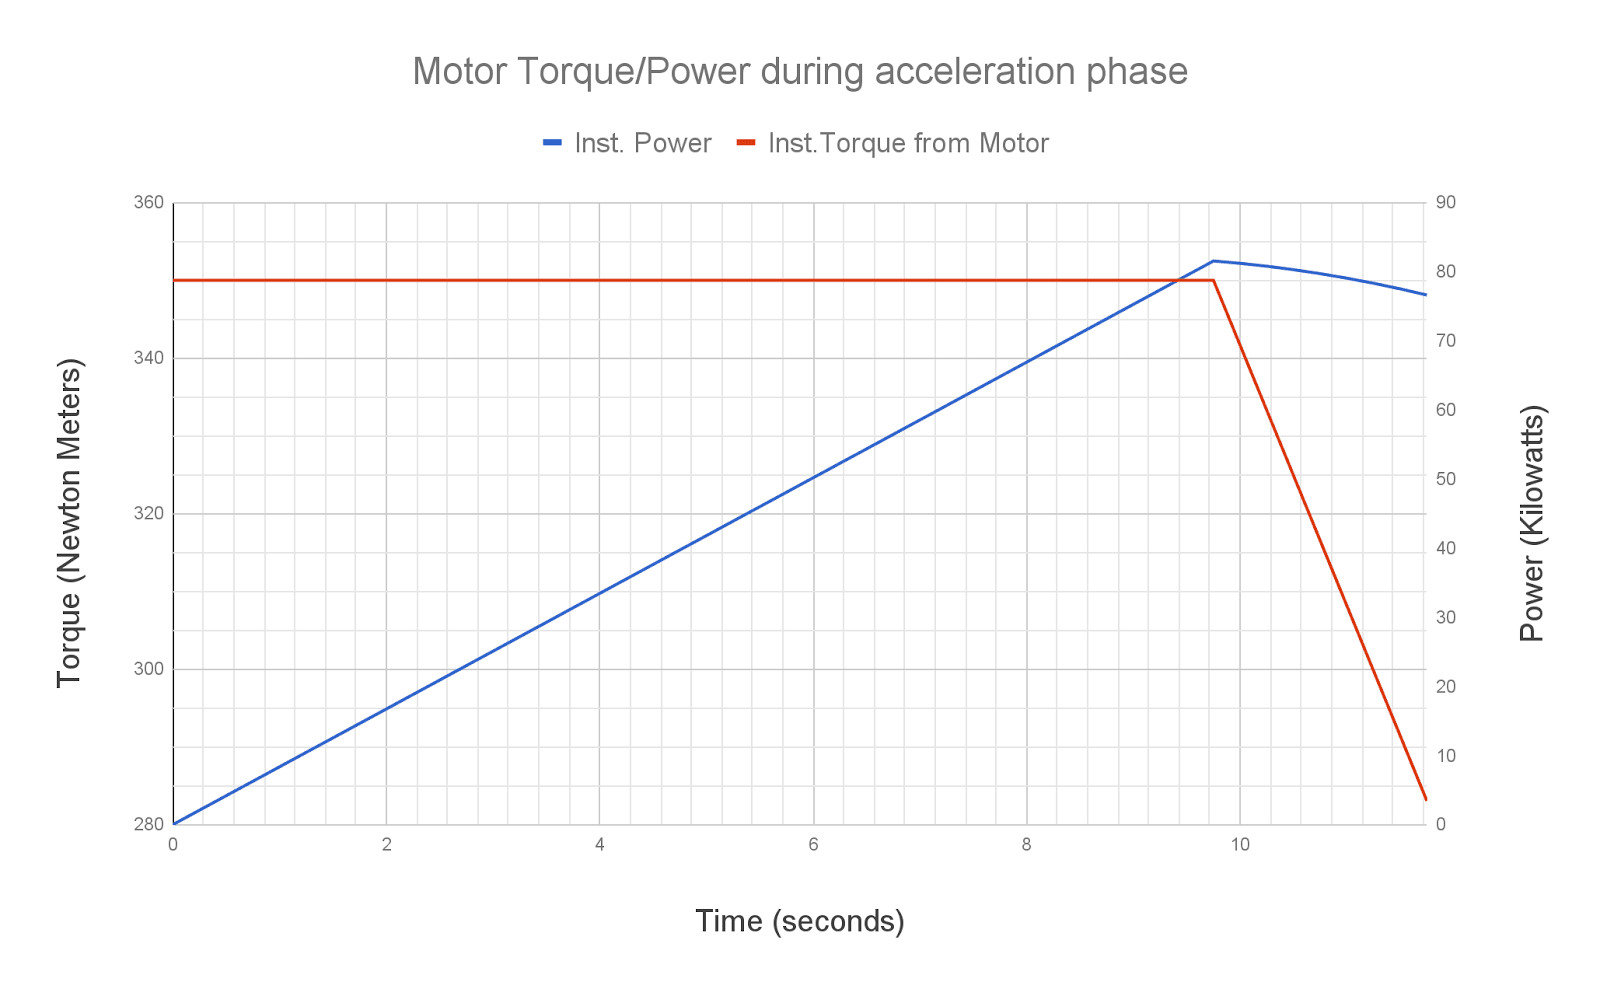
\includegraphics[width=\linewidth]{images/fig10}
        \caption{Motor Torque/Power during acceleration phase}
    \end{figure}
    \begin{figure}[H]
        \centering
        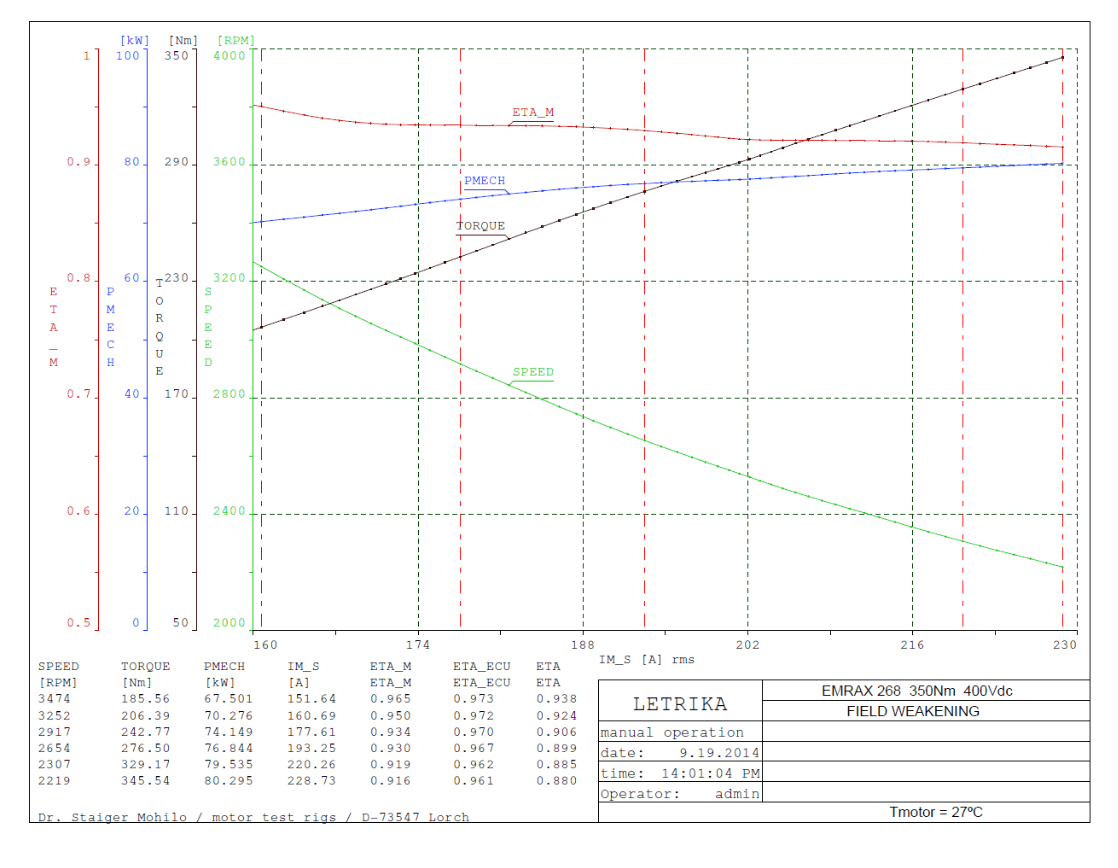
\includegraphics[width=\linewidth]{images/fig11}
        \caption{Caption needed}
    \end{figure}
    \subsection{Power Delivery}
    The EMRAX 268 has a variety of shaft mounting solutions. The most practiced ones are bolted flange shafts or a shaft within the splined hub of the motor. The flanged shaft was the choice for the design because of the ease at which one can assemble and perform maintenance on the powertrain and the versatility to alter shaft lengths and dimensions. In addition, in order to secure pulleys onto this shaft, the option of splining a shaft is available, which provides the most secure and efficient method of securing the pulleys. The shaft is made out of hardened steel (42CrMo4QT) which is commonly used to make driveshafts, turbocharger gears, crankshafts, etc.
    \begin{figure}[H]
        \centering
        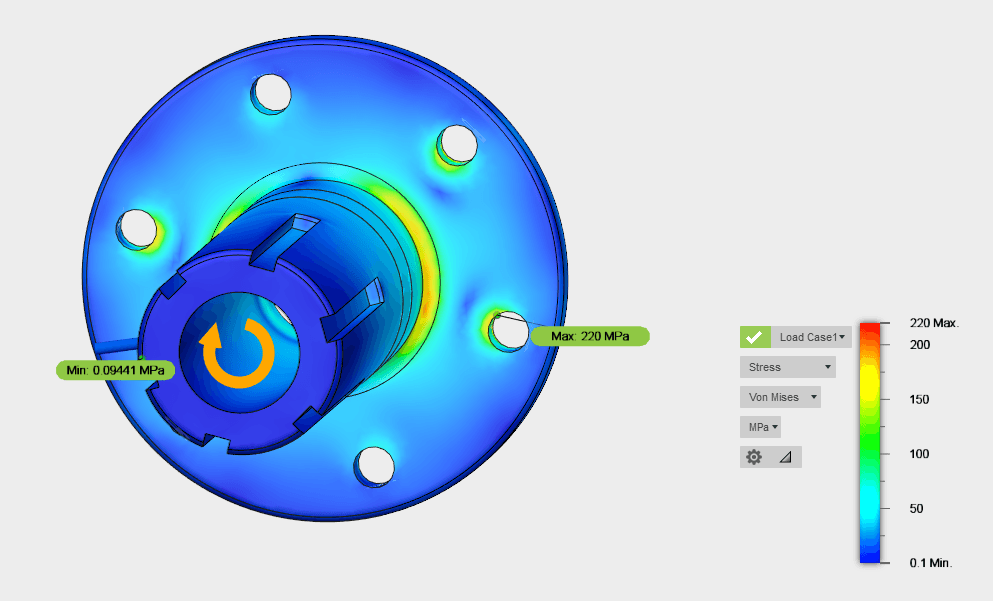
\includegraphics[width=\linewidth]{images/fig12}
        \caption{Caption needed}
    \end{figure}
    \subsubsection{Motor Shaft}
    Static stress FEA was done, in Autodesk Fusion 360, on the shaft in order to analyze stress concentrations and possible failures. The shaft was fixed via the bolt holes within the flange and the load was equivalent to the tension force that the pulley and belt system would exhibit at peak loads. In addition, an angular load was placed onto the shaft, equivalent to the maximum possible RPM range the motor could produce, which is about 1000 rad/s.\\

    The shaft experiences a peak stress of 220 MPa, located at the bolt holes on the flange. This raises concern regarding bolts that fasten the shaft to the motor. Reaction force was measured to be a peak of around 400N on the bolt, which means based on the cross sectional area of the bolt, shear force and moment, it would experience a peak of 338 MPa. This is within the yield strength of the bolt which is >965 MPa yield strength, exhibiting a safety factor around 3.
    \begin{figure}[H]
        \centering
        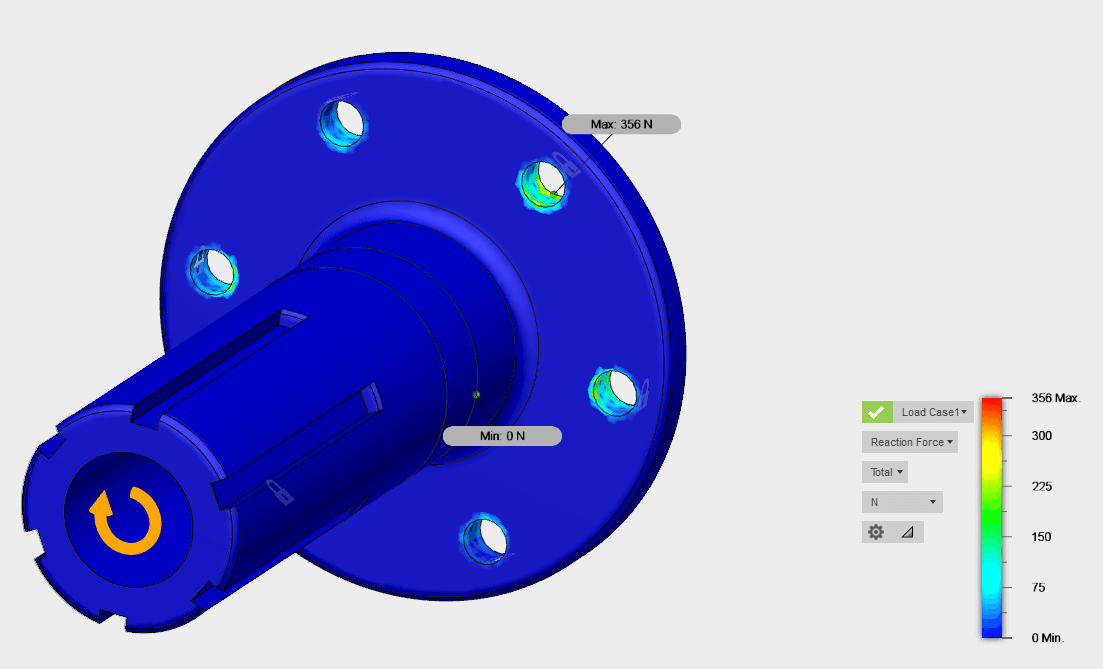
\includegraphics[width=\linewidth]{images/fig13}
        \caption{Caption needed}
    \end{figure}
    \begin{figure}[H]
        \centering
        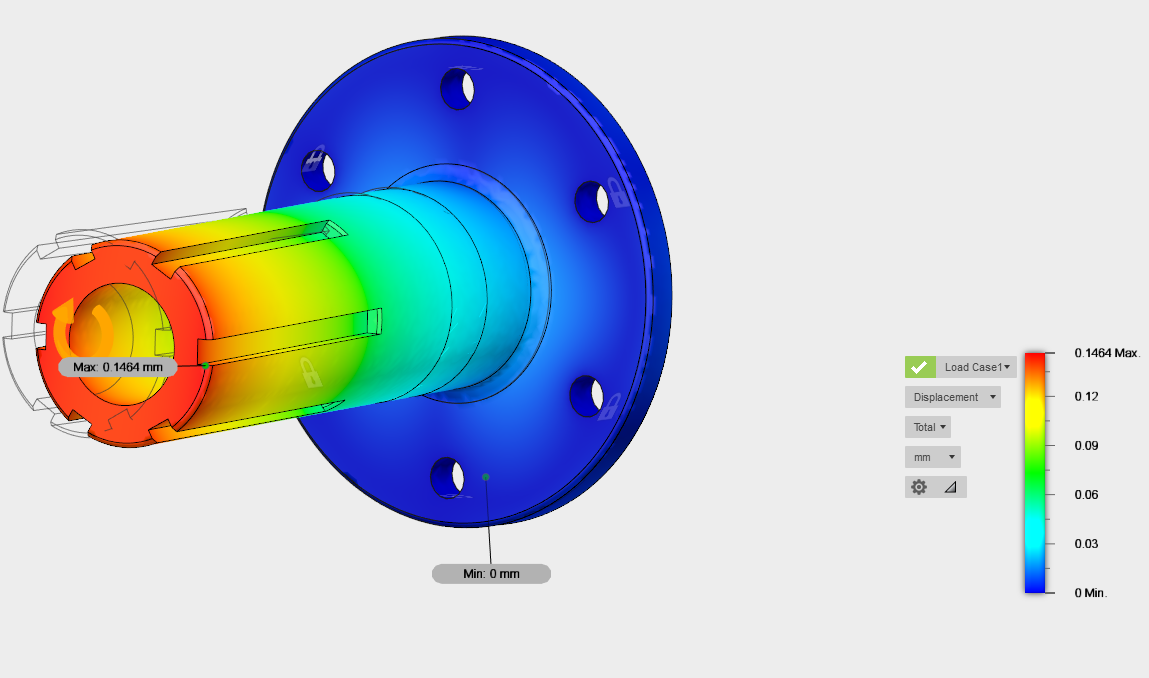
\includegraphics[width=\linewidth]{images/fig14}
        \caption{Caption needed}
    \end{figure}
    This is the displacement result of the FEA, where the peak displacement of the shaft is 0.15mm at the tip of the shaft. In the figure above, it is at a 5\% model based displacement adjustment. The mesh was created with an average element size of 3\% of the model based size had a parabolic element order. To refine our mesh and create more accurate results, adaptive mesh refinement was done in the areas of peak stress, at a cycle of 3 mesh refinements with a convergence tolerance of 5\%. Similar FEA was done on the other power transmission shaft that connects to the wheel. The result yielded less overall stress on the bolt holes due the shaft not having a hollowed core (200 MPa)
    \begin{figure}[H]
        \centering
        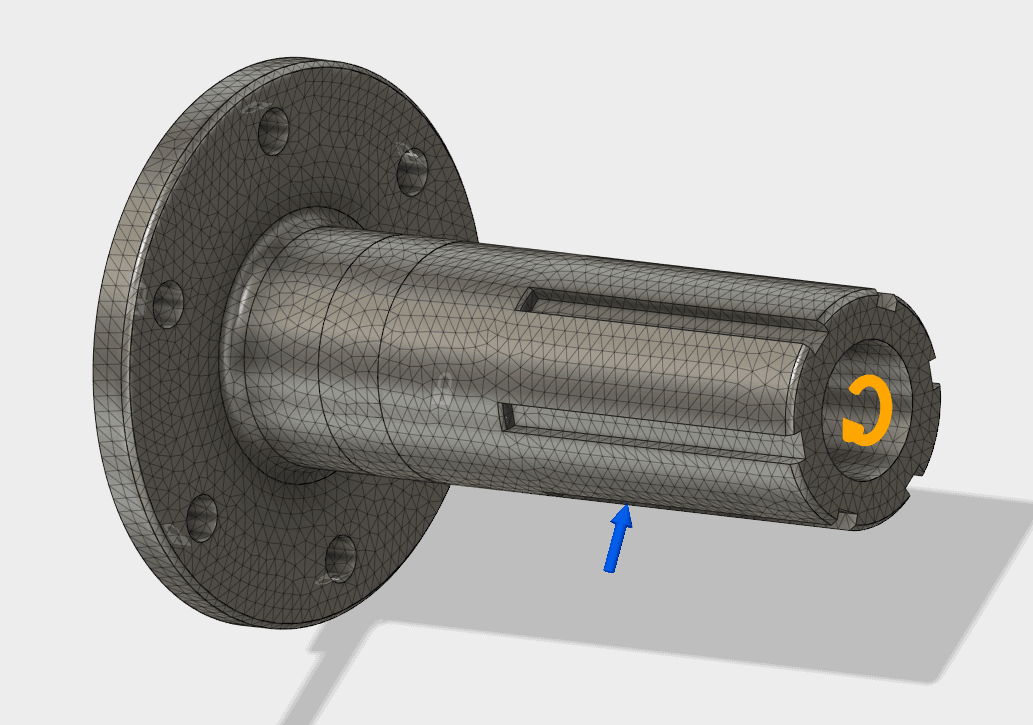
\includegraphics[width=\linewidth]{images/fig15}
        \caption{Caption needed}
    \end{figure}
    The mesh was created with an average element size of 3\% of the model based size had a parabolic element order. To refine our mesh and create more accurate results, adaptive mesh refinement was done in the areas of peak stress, at a cycle of 4 mesh refinements with a convergence tolerance of 5\%.

    \subsubsection{Pulley}
    \begin{figure}[H]
        \centering
        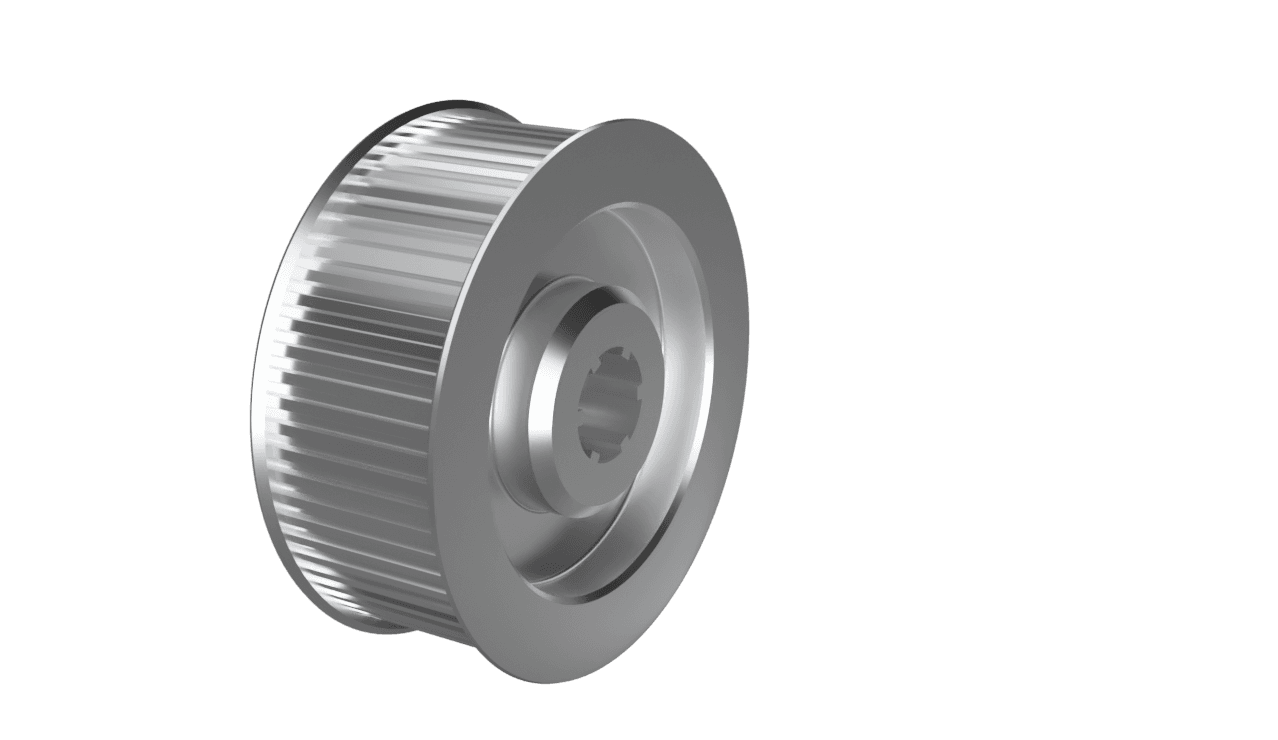
\includegraphics[width=\linewidth]{images/fig16}
        \caption{Caption needed}
    \end{figure}
    The propulsion system utilizes a single gear reduction in an open belt system, that incorporates an idler pulley to maintain contain tension on the system. Many different power transmission options were investigated, including a multi-gear system and a continuously variable transmission (CVT) system. However, these options were not chosen due to the overall complexity that these systems would have, and the costs and research \& development time involved in developing these systems would be far beyond the timeline allocated by the competition. Thus, a single gear reduction with the open belt system was chosen for the simplicity of design and testing, and the reduction of overall costs in integrated this power transmission system onto the pod.

    \paragraph{Vacuum Compatibility}
    We have identified two potential issues with the motor in vacuum, which we have discussed with the manufacturer EMRAX.
    \begin{itemize}
        \item Cooling of the motor may be designed for air environments, where air convection plays a role in addition to the liquid cooling system.
        \begin{itemize}
            \item EMRAX believes that due to the very short runtime (less than 30 seconds) there will be no significant difference in the efficacy of the cooling system in vacuum.
            \item They have also suggested that no cooling system is needed at all, and the heat capacity of the motor itself is enough to last 30 seconds without reaching 50 degrees Celsius. We decided to design a cooling system anyway, on the grounds that it would be prudent to have and could be relatively trivially removed if physical tests showed it to be significantly redundant.
        \end{itemize}
        \item Outgassing of the epoxy used to secure the motor’s internal components could weaken these fastenings and also deposit epoxy on other parts of the motor.
        \begin{itemize}
            \item EMRAX has confirmed that the motor’s internal components are both mechanically and chemically secured, so that even with epoxy outgassing there will be no problems in fastening.
            \item Deposition of epoxy could damage other parts within the motor. [CAN WE ASK THEM WHAT THINGS THEY ARE USING THAT COULD OUTGAS?]
        \end{itemize}
    \end{itemize}

    \subsection{ESC}
    EMRAX recommended several electronic speed controllers (ESC) and the UniTek Bamocar D3 stood out due to its low-cost and well-balanced performance. The controller weighs 6.8 kilograms and accepts a voltage input of up to 700 V, with a continuous current of 200 A. The controller also comes with a liquid cooling system that is situated at the bottom of the controller.
    \begin{figure}[H]
        \centering
        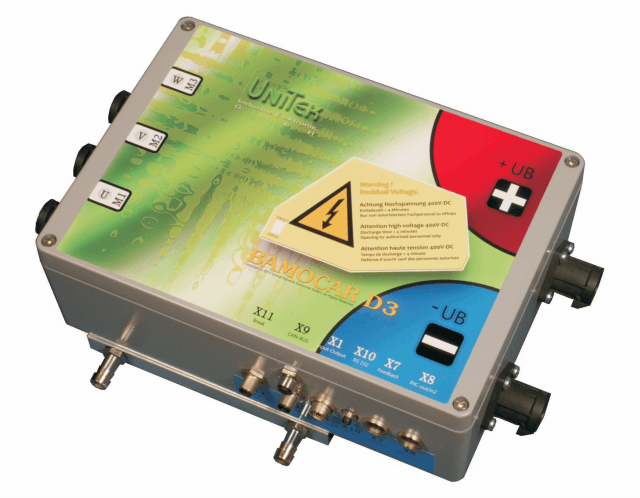
\includegraphics[width=\linewidth]{images/fig17}
        \caption{Caption needed}
    \end{figure}

    \subsection{Cooling System}
    Cooling system; heat transfer calcs results; thermal simulation would be nice [including ESC and motor]\\

    The cooling system is designed to be as safe as possible by offering ample cooling while also making it easy to assemble and maintain. The EMRAX 268 specifies limits to the flow rate and pressure of the cooling loop with a flow rate of 8 litres per minute at 2 bars accounting for vacuum, the loop will be running at 7 litres per minute at 1.5 bars to stay under these limits. The cooling loop(figure ?) is a series loop with no parallel lanes, allowing for a simple to install and clean path for a 25/75 glycol/water solution as coolant. The loop will be using multiple temperature and pressure sensors to ensure the coolant will never exceed the pressure or temperature limit of the motor of 2 Bar and motor inlet coolant temperature of \SI{50}{\celsius}. If the 2 bar pressure limit is reached, a solenoid valve will be opened to release some coolant into a release tank, allowing pressure inside the cooling loop to be lowered. In the event of the temperature limit being reached, the motor and controller settings will be lowered to allow for heat to be dissipated from the loop and the temperature to be lowered. A ball valve is also present in order to completely stop the flow of coolant when the power is off and the pod is not running.
    \begin{figure}[H]
        \centering
        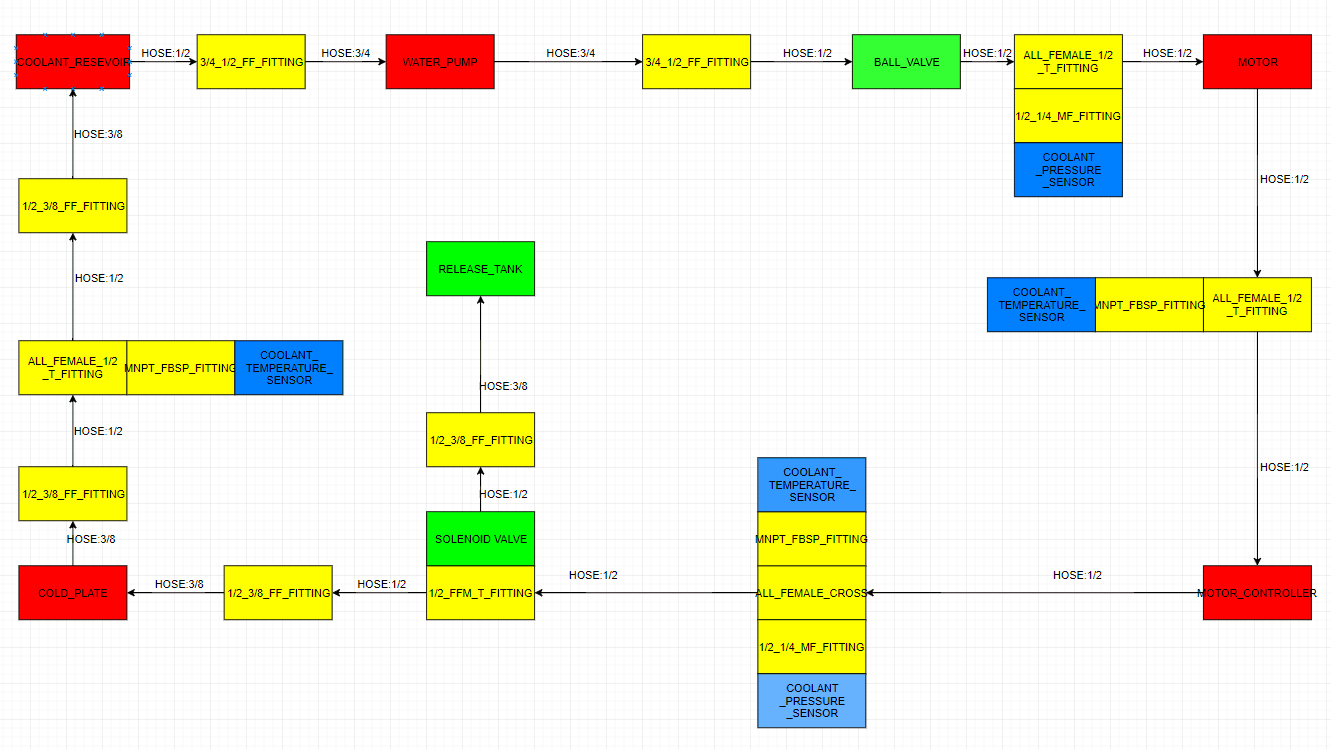
\includegraphics[width=\linewidth]{images/fig18}
        \caption{The cooling loop uses fittings and hoses in order to move from one component to the next seamlessly}
    \end{figure}
    The design parameters of the cooling system used worst-case-scenario heat dissipation numbers: the motor uses 100 kW at peak, with specified minimum 92\% efficiency, with the motor controller introducing a maximum of 3 kW,  so we must dissipate 11 kW during a maximum run time of 20 seconds. Using these values and assuming no heat is dissipated through the cold plate and tubing, the total heat input to the loop was calculated using
    \[
    Q = mc \Delta T
    \]
    where $Q$ is \SI{220}{kJ}, $c$ is \SI{3.85}{kJ/kgK} for a 25/75 water/glycol solution at \SI{25}{\celsius}, $m$ is mass of coolant required, and $\Delta T$ is \SI{25}{\celsius}. The mass of coolant required is approximately \SI{2.3}{kg} or $\sim$\SI{2.3}{L}. A 2 litre reservoir was chosen to make up most of the required coolant with the volume of the tubing adding the rest and more. In addition, a cold plate is present in the loop as another safety and redundancy factor in the loop. With the tubing and cold plate dissipating heat, an extra 5 seconds of expected run time, and supplementary coolant mass, it can be estimated that the cooling loop will not exceed a delta temperature of \SI{25}{\celsius}, allowing for a safe acceleration and run of the pod.\\

    The cold plate will be attached to a beam on the ladder frame of the pod, acting as a metal block to absorb any heat that is created. With temperatures not exceeding \SI{50}{\celsius} in the loop before the addition of the coldplate, the aluminum beam will not experience any extreme heat, keeping the integrity of the frame and pod.

    \subsection{Wheel \& Slip}
    Wheel material, cost, fabrication (how are we doing polyurethane?)
    \begin{figure}[H]
        \centering
        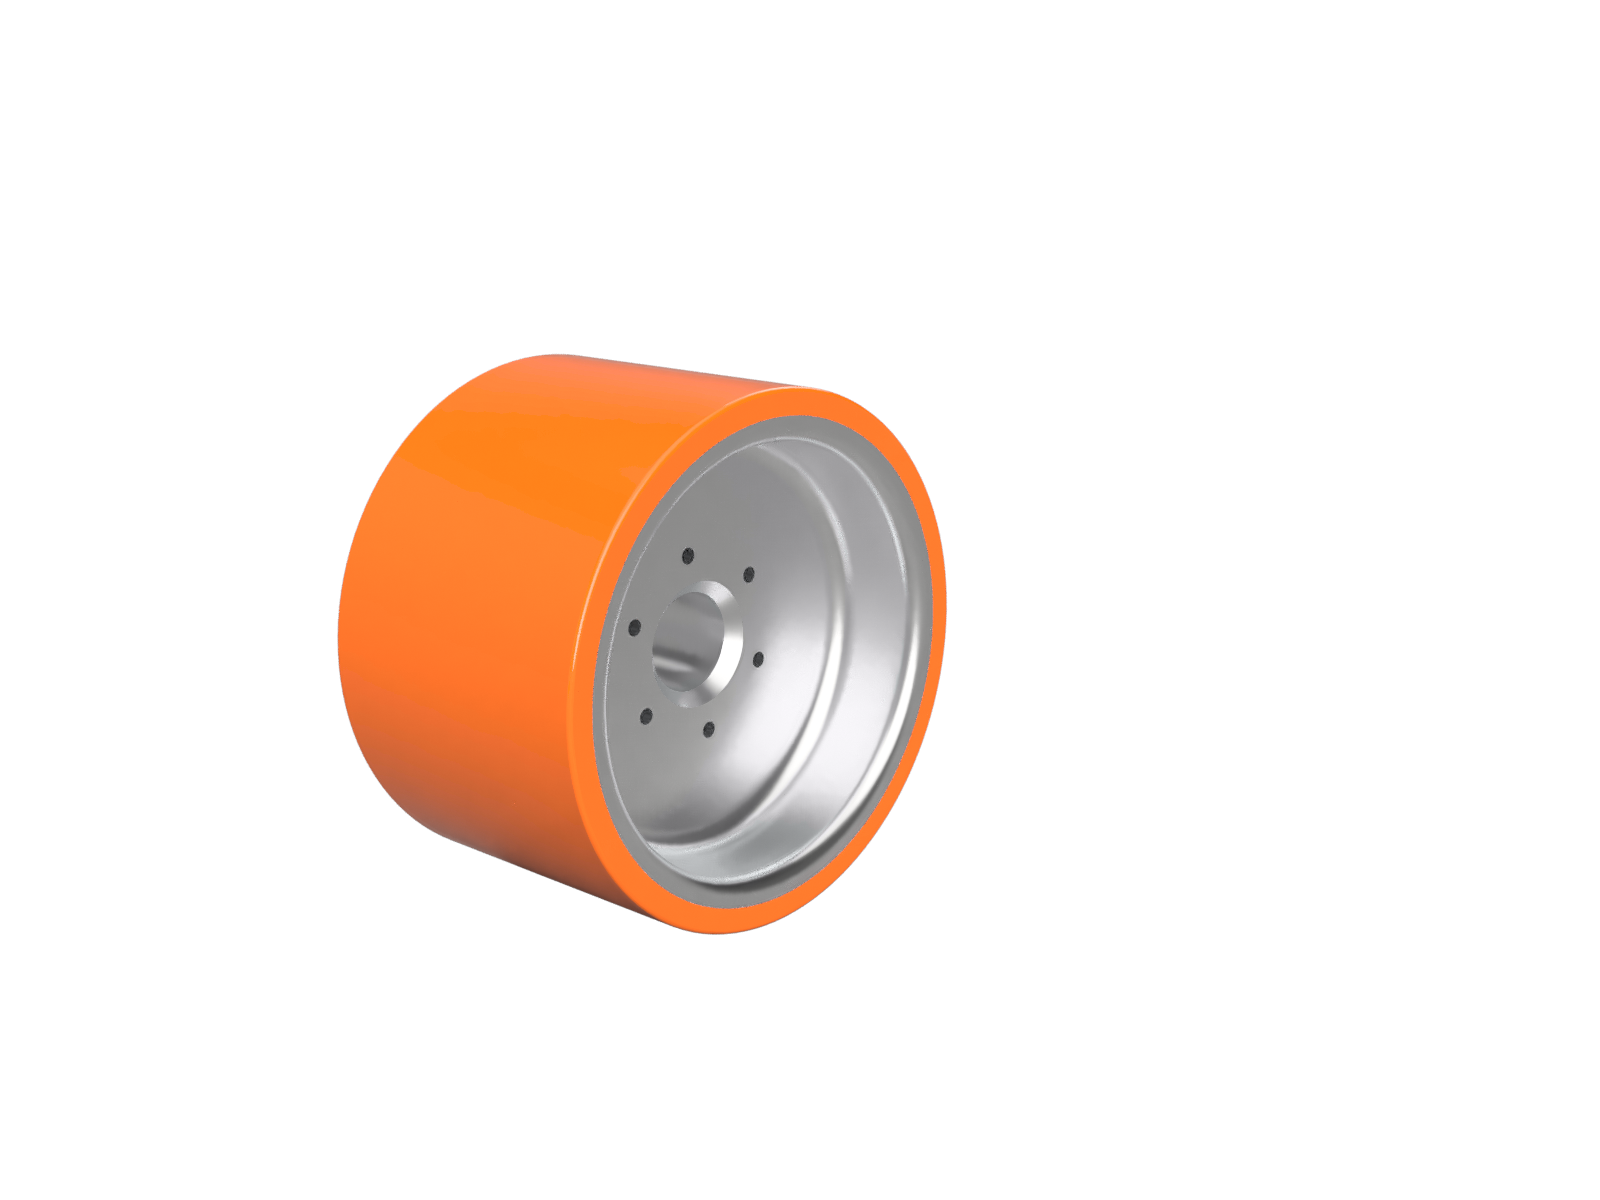
\includegraphics[width=\linewidth]{images/fig19}
        \caption{Caption needed}
    \end{figure}
    Our propulsion system requires strong wheels that are able to withstand high RPM ranges at a large variety of axial and thrust loads. The design was created with an aluminum 6061-T6511 core and a polyurethane wheel tread. Aluminium 6061-T6511 was chosen as the wheel’s core because of the yield strength and low density as we would require the wheel to be lightweight in order to minimize inefficiency of transferring torque to the ground and the strength such that the wheel will not yield under peak loads. In addition, because this material is easily machined, there is no need for extensive tooling or custom extrusion techniques in order to produce the wheel. 6061-T6511 is a well known and common alloy and thus extensive research has been conducted on the fatigue behaviour of this wheel. Based on fatigue analysis\footnote{ https://www.osti.gov/scitech/servlets/purl/10157028}, even when the wheel has done $10^6$ cycles, it will still be within design specifications and can be used safely.\\

    Testing for the wheel (balance issues?)

    \paragraph{Calculations for slip}
    By using first-principles of newtonian physics, we can simplify our traction based on static friction. In order to translate angular movement into translational movement, we require that the wheel remain in traction with the track.\\

    Where the overall mass, $m$, of the pod is \SI{150}{kg} and 65\% of the weight is biased towards the drive wheel.

    \begin{center}
        We want to achieve an acceleration of \SI{1}{g} or \SI{9.8}{m/s^2}\\

        Thus, $F_a=m\cdot a = \SI{150}{kg} \times \SI{9.8}{m/s^2} = \SI{1500}{N}$\\

        Frictional force is calculated via $F_f=\mu_s \times F_n$. In this case, $F_f=F_a=\SI{1500}{N}$\\

        Based on the static coefficient of friction of 0.7 with polyurethane vs aluminum,
        \[
        F_n = \frac{F_f}{\mu_s} = \frac{\SI{1500}{N}}{0.7} \approx \SI{2200}{N}
        \]

        But with 65\% biased on the drive wheel, only $\SI{1500}{N} \times 0.6 = \SI{975}{N}$\\

        But we have a deficit in normal force. $\SI{2200}{N} -\SI{975}{N}=\SI{1225}{N}$
    \end{center}
    Based on these calculations, we required that we increase the normal force between the wheel and the rail in order to achieve our nominal acceleration of around 1 g and to prevent slipping of the drive wheel.\\

    The wheel core will be machined from an aluminum billet on a CNC. This will be fairly simple to achieve, and does not require any special tooling or machining processes to accomplish. In addition, this allows the balancing of the wheel to be easily achievable due to the lack of manufacturing errors that are produced by casting the wheel. In order to produce the polyurethane tread, we must create a mold and cast the polyurethane tread. This tread will then be chemically secured to the aluminum wheel via vacuum grade epoxy. This process takes the majority of the cost associated with producing the wheel- however, the possibility of machining the tread out of a solid block of polyurethane is currently being investigated as it as a vastly more cost effective solution.

    A solution to our normal force deficit: Pneumatic Actuators
    \begin{figure}[H]
        \centering
        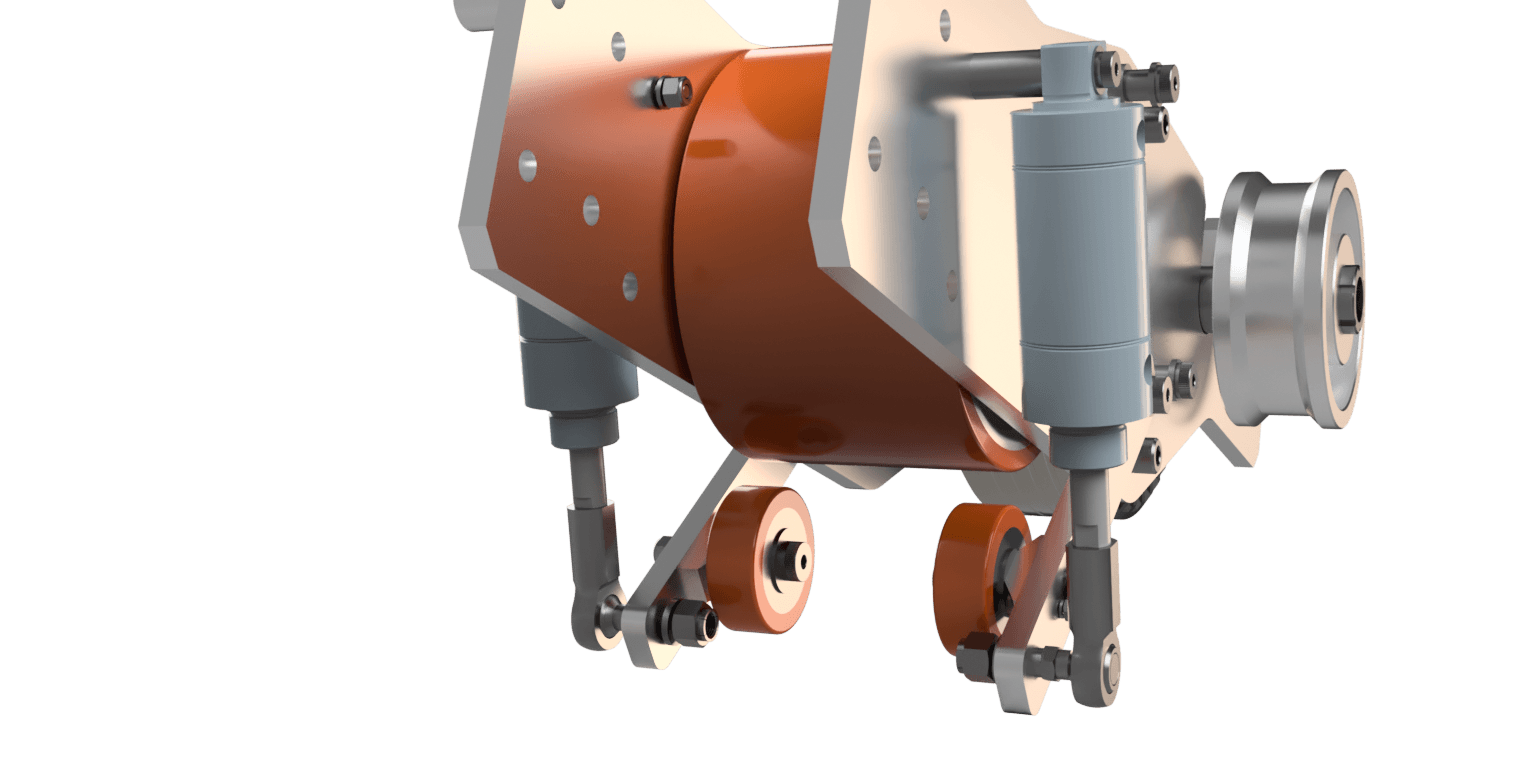
\includegraphics[width=\linewidth]{images/fig20}
        \caption{Caption needed}
    \end{figure}
    By utilising a guide wheel under the I-beam and a pneumatic actuator fastened to a pivot arm to clamp down onto the I-beam flange, we are able to increase the theoretical normal force that the wheel can provide and thus increase our static frictional force. The pneumatic actuator allows us to modulate the traction force needed and dampen any impacts that the guide wheels will encounter moving down the track.

    \paragraph{Pneumatic Circuit}
    Is there a way to do both centripetal and shear FEA on the polyurethane?\\
    \begin{figure}[H]
        \centering
        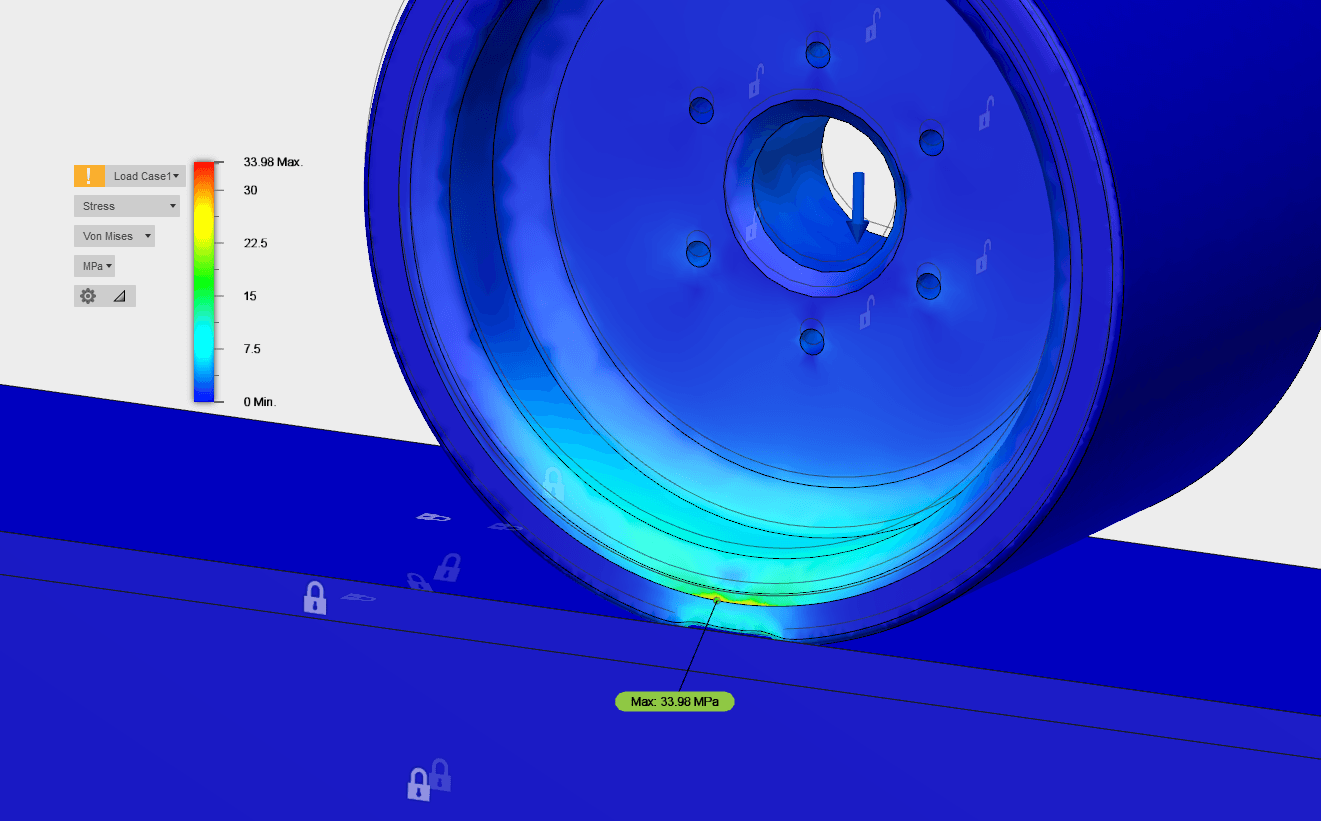
\includegraphics[width=\linewidth]{images/fig21}
        \caption{Static Stress FEA, Peak compressive load on main drive wheel}
    \end{figure}
    This finite element analysis was conducted, in Autodesk Fusion 360, by placing a compressive load onto the wheel equivalent to the weight of the pod, plus the force that the pneumatic actuators would provide in order to create the required traction force. The track was grounded and fixed in all orthogonal directions and the wheel fixed via the bolt fixtures within the aluminum core.\\

    The aluminum core only experiences a peak stress of \SI{34}{MPa}, which is significantly lower than the yield strength of the material, \SI{275}{MPa}, and provides a safety factor of over 8. The polyurethane tread is a hardness of \SI{90}{A} on the Shore hardness scale. The tread experiences a peak stress of \SI{17}{MPa}, where as the tensile strength of the tread material is \SI{50}{MPa}, giving us a suitable safety factor of around 3.
    \begin{figure}[H]
        \centering
        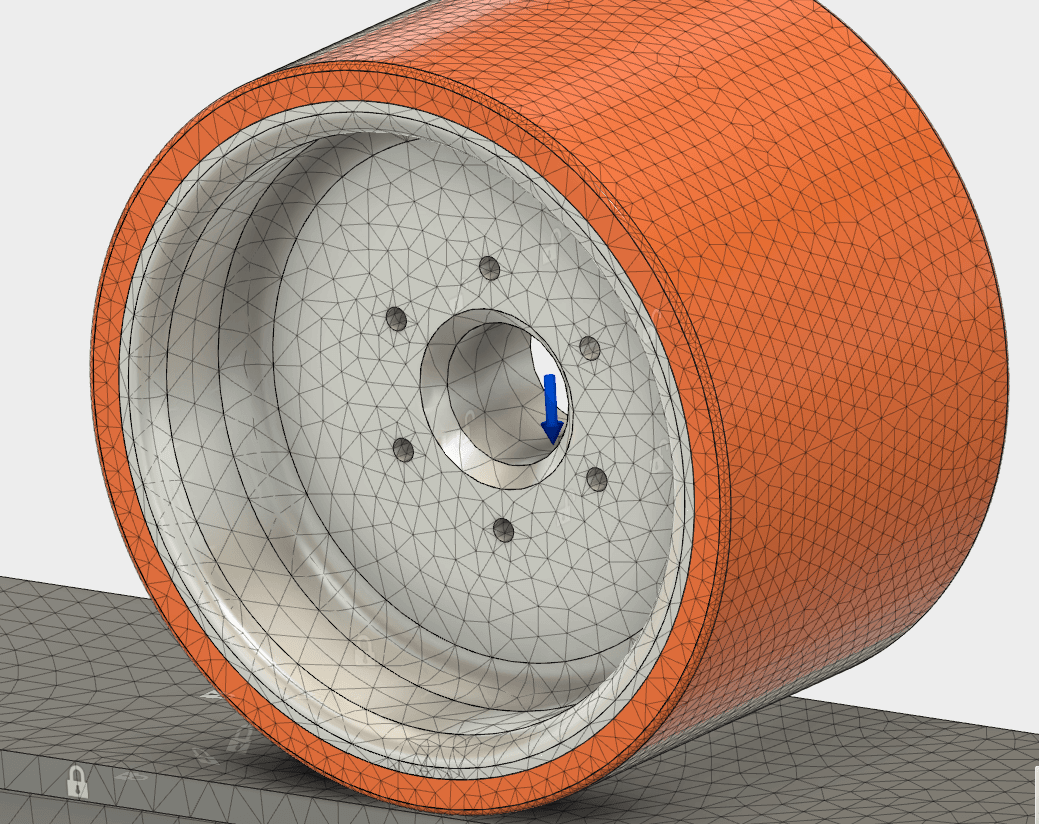
\includegraphics[width=\linewidth]{images/fig22}
        \caption{Caption needed}
    \end{figure}
    The mesh was created with an average element size of 2\% of the model based size had a parabolic element order. To refine our mesh and create more accurate results, adaptive mesh refinement was done in the areas of peak stress, at a cycle of 6 mesh refinements with a convergence tolerance of 5\%.

    \paragraph{Wheel balancing}
    \subsection{Friction Braking Calipers}
    \begin{figure}[H]
        \centering
        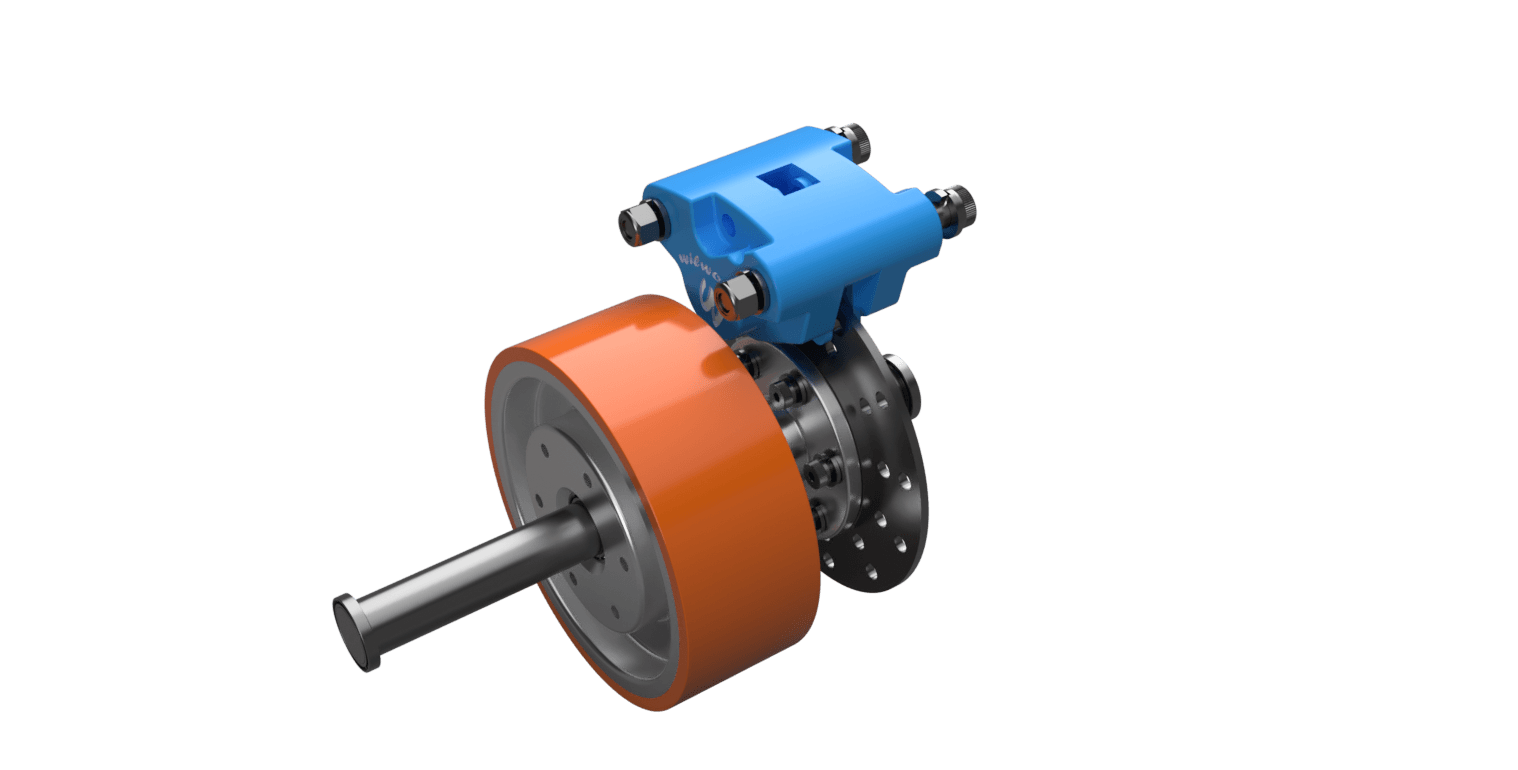
\includegraphics[width=\linewidth]{images/fig23}
        \caption{Caption needed}
    \end{figure}

    \paragraph{Motivation}
    Due to Eddy Current Brakes (see below) being ineffective at speeds below 5 m/s, the pod required a secondary braking source to bring it to a complete stop. Friction brake calipers were determined to be the most simple and effective solution, with many off-the-shelf components available. The brakes are not required to perform at high speeds, and as such, do not require large brake rotors or high performance calipers/pads in order to stop the vehicle  As such, there is no requirement to create a custom braking system and the cost associated with creating such a braking system are minimal. It is easily integrated into the original design, requiring little to no alteration to major drivetrain components.\\

    \paragraph{Heating}
    The kinetic energy before friction brake is activated is given by: $\frac{1}{2}mv^2=12(150)(10)^2=\SI{1875}{J}$\\
    When the friction brake is activated, kinetic energy will be converted to heat, which will be transferred to the brake rotor disc and the brake pad.
    Although the manufacturer did not specifically state the material composition, gray cast iron is the most common material for brake rotor discs. A rough estimation of the composition of such material, and the density and specific heat capacity of each metallic element, are as follows:\\

    \begin{table}[H]
        \centering
        \begin{tabular}{@{}lrrrrrr@{}} \toprule
            Element & Iron & Carbon & Silicon & Manganese & Phosphorus & Sulfur\\ \midrule
            \% Weight & 93.487\% & 3.4\% & 2\% & 0.58\% & 0.51\% & 0.023\%\\
            Density (\si{g/mm^3}) & 0.007874 & 0.00226 & 0.00233 & 0.00747 & 0.00196 & 0.001823\\
            Specific Heat Capacity (\si{J/(g\celsius)}) & 0.449 & 0.71 & 0.71 & 0.479 & 0.705 & 0.770\\ \bottomrule
        \end{tabular}
        \caption{Caption needed}
    \end{table}

    Using the dimensions provided by the manufacturer, the volume of the brake rotor disc can be found.
    \[
    4\pi(63)^2-\pi(23.5)^2-120\pi(3.175)^2=\SI{44340}{mm^3}
    \]
    The mass and specific heat capacity of the brake rotor disc can be found using the percentage weight, density and specific heat capacity of each element.
    \begin{gather*}
    \mathrm{Mass} = \frac{44340}{\frac{0.034}{0.00226} + \frac{0.02}{0.00233} + \frac{0.0058}{0.00747} + \frac{0.0051}{0.00196} + \frac{0.00023}{0.001823} + \frac{0.93487}{0.007874}} = \SI{303.6}{g}\\
    \textit{SHC}=0.71(0.034)+0.71(0.02)+0.479(0.0058)+0.705(0.0051)+0.770(0.00023)+0.449(0.93487)=0.465
    \end{gather*}
    Although the brake pad uses sintered metallic material, the material composition is kept confidential by the manufacturer. The composition is drastically different between manufacturers, thus it is rather hard to make an appropriate estimation. Some of the common primary materials are graphite, copper and iron. Carbon steel serves as a decent balance among the three materials, and thus is used to make an approximation.\\

    The density of carbon steel is \SI{0.00785}{g/mm^3}, with a specific heat capacity of \SI{0.49}{J/(g\celsius)}. The volume of the brake pad is \SI{5572}{mm3}, which approximates the mass to be \SI{43.7}{g}.

    Using the heat transfer equation of $\Delta Q = mc \Delta T$,
    \[
    T=\frac{1875}{303.6(0.465)+43.7(0.49)}=\SI{11.5}{\celsius}
    \]
    The brake rotor disc and the brake pad will gain approximately \SI{1875}{J} of energy, and the temperature will increase by \SI{11.5}{\celsius}.\\

    https://willmanind.com/what-is-grey-cast-iron/\\
    http://periodictable.com/Properties/A/Density.al.html\\
    http://periodictable.com/Properties/A/SpecificHeat.html

    \paragraph{Failsafes}
    The solenoid that controls the brake master cylinder will be on an electrically failsafe circuit, in the case of power loss, there will be a reserved battery source to make sure that the calipers are actuated at the correct speeds. In addition, these brakes are mechanically failsafe. In the case of complete electrical power loss, the solenoid holding the calipers opens will be a normally open valve and will automatically actuate.

    \subsection{Tests \& Validation (completed and planned)}
    Test rig (see Next Steps as well)\\
    Fault tolerance, potential failure modes (FMEA)\\
    How will we verify that the OTS motor is in fact working to spec?\\
    How will we test all aspects of the motor?

\end{document}
